\documentclass[a4paper,11pt,titlepage]{article}
\usepackage[utf8]{inputenc}
\usepackage{amsmath, amssymb}
\usepackage{graphicx}
\usepackage{hyperref}
\usepackage{geometry}
\usepackage{float}
\usepackage{cite}

\geometry{margin=1in}

\title{\Huge \textbf{GIC 2026: Quantum-Enhanced Microgrid BESS Siting} \\
\Large IEEE 33-Bus System Optimization Report}
\author{\textbf{Abdullah Al Omar Galib}}
\date{\today}

\begin{document}

\maketitle
\thispagestyle{empty}
\newpage

\tableofcontents
\listoffigures
\newpage

\section{Introduction and Problem Statement}
Strategic siting of Battery Energy Storage Systems (BESS) in distribution networks is critical for enhancing grid stability, resilience, and economic efficiency. The IEEE 33-bus system \cite{baran1989network} provides an industry-standard radial network benchmark. Siting optimization is naturally modeled as an NP-hard combinatorial mixed-integer program, where the search space grows exponentially with the network size.

This report documents the workflow and mathematical approach utilizing the Quantum Approximate Optimization Algorithm (QAOA) \cite{farhi2014quantum} implemented via Qiskit \cite{qiskit2023}, mapped against exact mathematical formulations and physically verified by standard classical bounds testing.

\section{Dataset and Cost Parameters}
We evaluate the BESS capital expenditures using authoritative data bounds from the US DOE NREL Annual Technology Baseline (ATB) 2024 repository \cite{mirletz2024atb}. The \texttt{2024\_v3\_Model\_Parameters.csv} dataset structure encompasses multiple parameters including \texttt{Technology} (e.g., Utility-Scale Battery Storage), \texttt{TechDetail} (e.g., 4-Hour duration), \texttt{Core Metric Parameter} (CAPEX, OPEX), \texttt{Scenario} (Moderate), \texttt{Year} (2024), and the corresponding numerical \texttt{Value}. This data is parsed to isolate precise 2024 CAPEX metrics for our model, bridging real-world economic constants with our quantum optimization constraints \cite{farhi2014quantum}.

\section{Grid State and Resilience Formulation}
The simulation utilizes the \texttt{pandapower} \cite{thurner2018pandapower} backward/forward sweep load flows to profile baseline grid degradation prior to the installation of storage elements.

\begin{figure}[H]
    \centering
    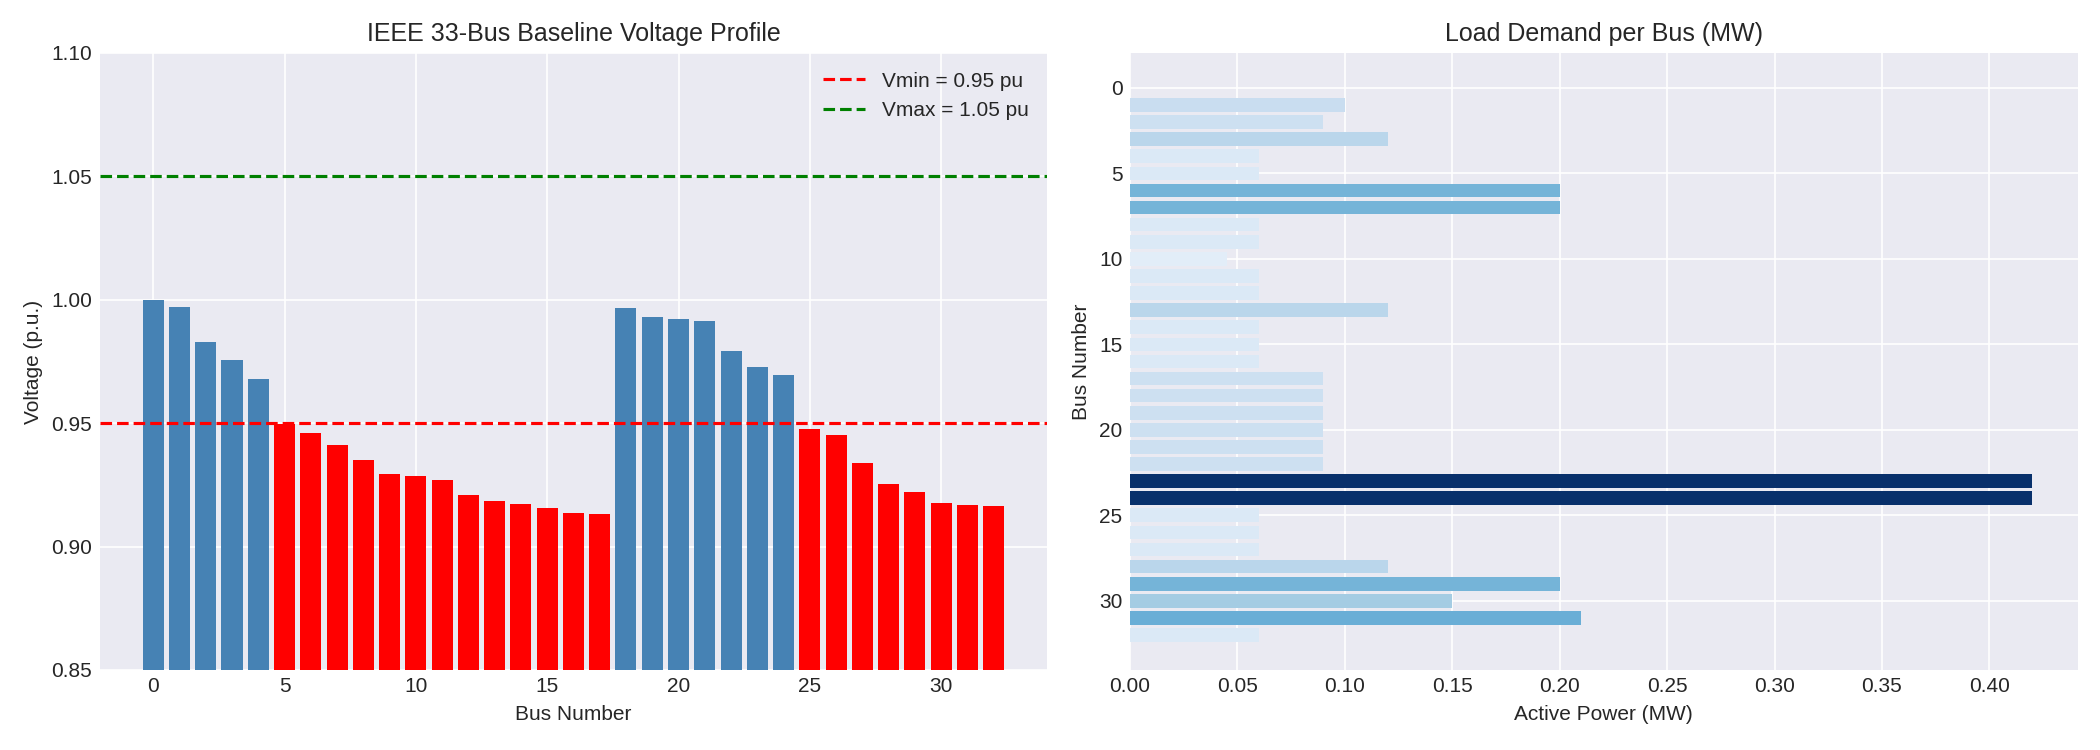
\includegraphics[width=0.95\columnwidth]{../images/01_baseline_grid.png}
    \caption{Baseline voltage profile and load demand for IEEE 33-bus network.}
\end{figure}

We defined a tri-component composite resilience score modeling topological importance, load density, and voltage deterioration gradients:

\begin{equation}
resilience\_score[i] = load\_demand[i] + 10 \times \max\left(0, 1.0 - baseline\_voltage[i]\right) + 2 \times \left(\frac{i}{33}\right)
\end{equation}

\begin{figure}[H]
    \centering
    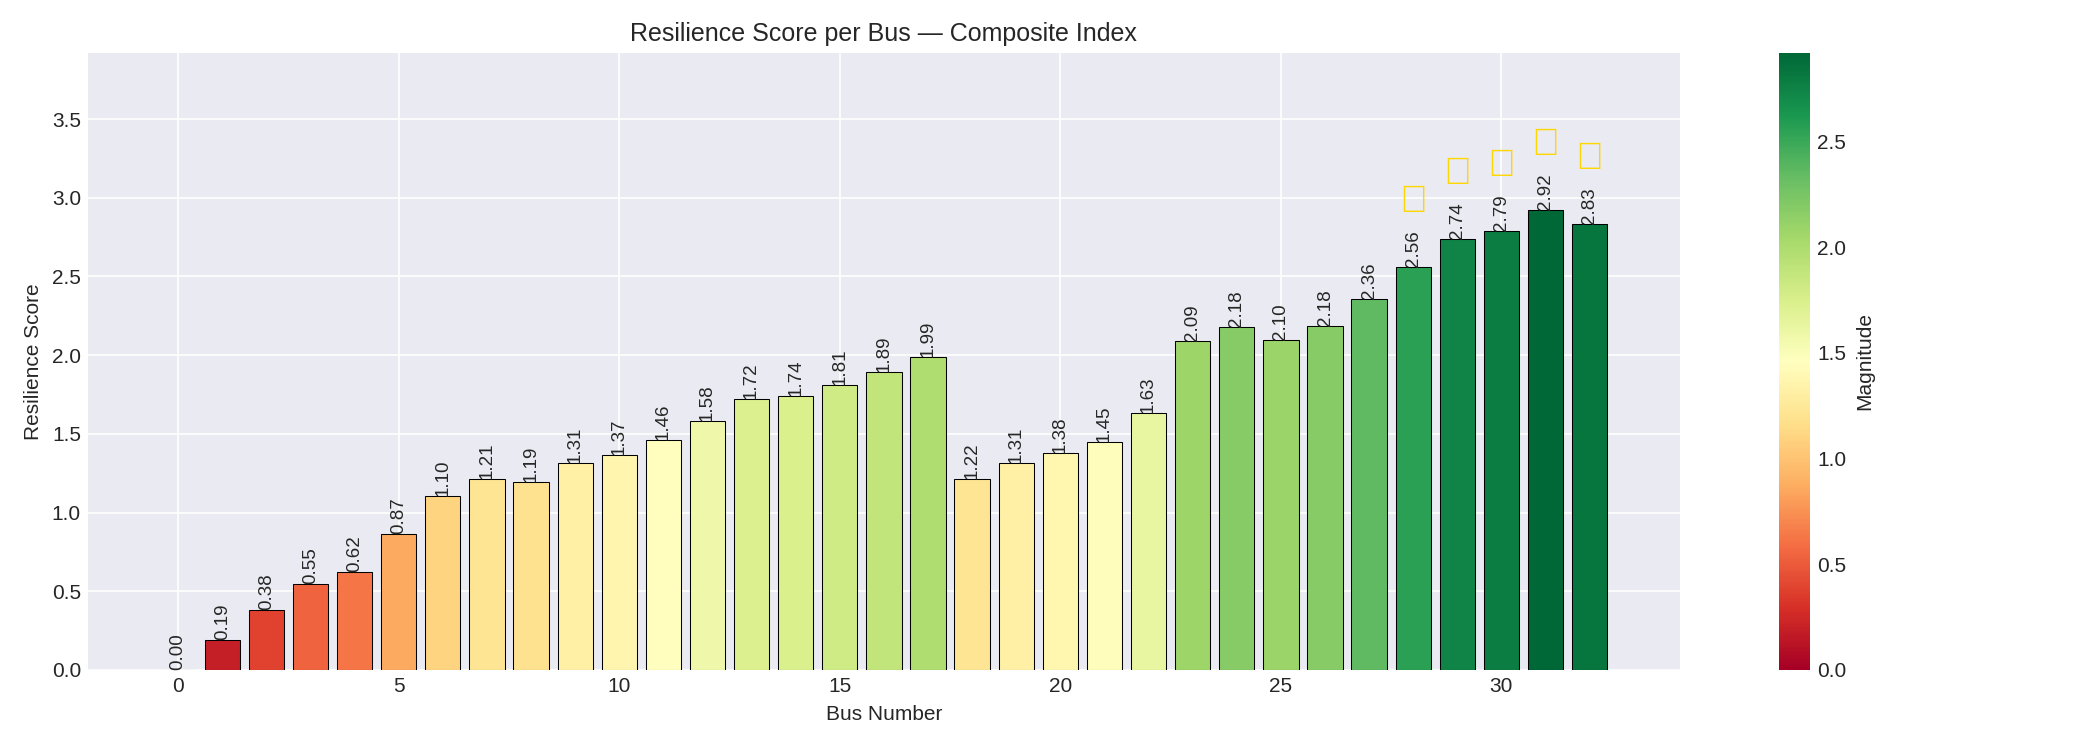
\includegraphics[width=0.95\columnwidth]{../images/02_resilience_scores.png}
    \caption{Aggregate network resilience values defining priority vectors.}
\end{figure}


\section{Binary Integer Program (BIP)}
BESS installation targets must balance capital expenditures (CAPEX, defined per NREL ATB 2024 Moderate scenario parameters, 4Hr scale) against cumulative resilience enhancements.

\subsection{Objective Function}
\begin{equation}
\min C(x) = \alpha \sum_{i=1}^{N} c_i x_i - \beta \sum_{i=1}^{N} r_i x_i
\end{equation}
Where:
\begin{itemize}
    \item $x_i \in \{0, 1\}$ dictates installation at bus index $i$.
    \item $\alpha = 0.5$ acts as the empirical cost weight penalty scalar.
    \item $\beta = 1.0$ controls proportional resilience maximization.
    \item $c_i$ is NREL's CAPEX bounds in $\$M$.
    \item $r_i$ corresponds to the resilience score vector per bus $i$.
\end{itemize}

\subsection{Budget Constraints}
Allocation is implicitly restricted to $K=5$ operational units across localized regions.
\begin{equation}
\sum_{i=1}^{N} x_i \leq K
\end{equation}

\begin{figure}[H]
    \centering
    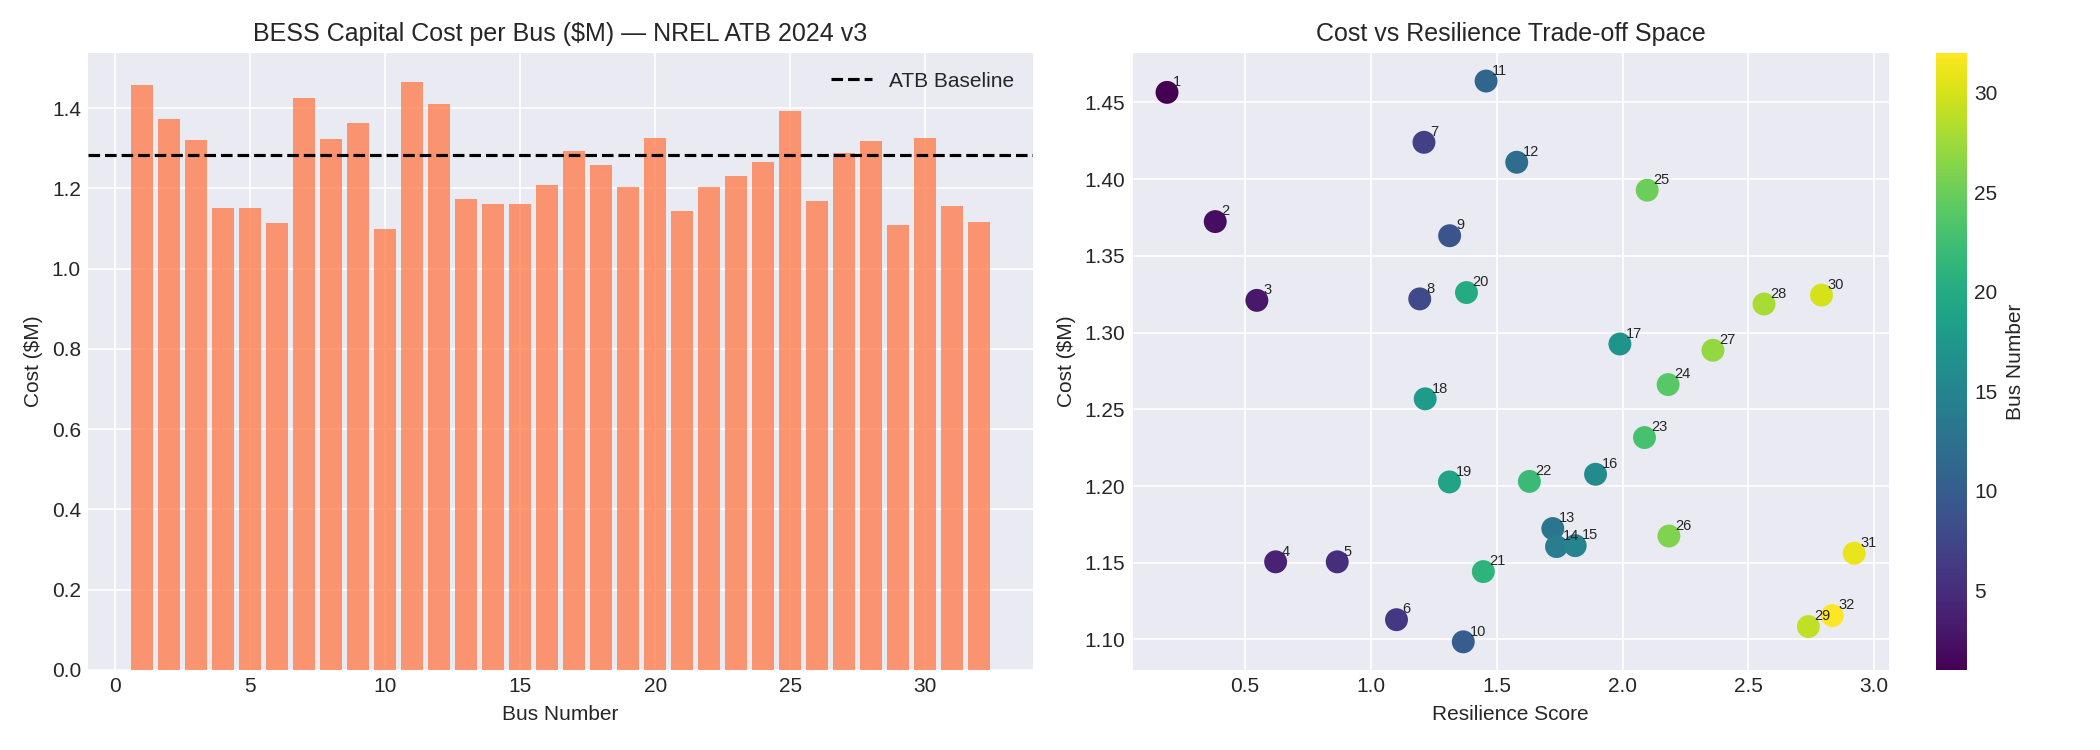
\includegraphics[width=0.95\columnwidth]{../images/03_cost_analysis.png}
    \caption{Physical installation cost correlations per node parameters.}
\end{figure}


\section{QUBO Mapping for the Quantum Target}
Inequality constraints formulated linearly cannot natively execute across Ising Hamiltonians. The capacity constraint $K$ is transformed into a bounding formulation via generalized quadratic penalty structures:

\begin{equation}
H_P = P \times \left(\sum_{i=1}^{N} x_i - K \right)^2
\end{equation}
Where $P = 20.0$ bounds strict feasibility ranges mathematically mapping:
\begin{equation}
Q_{ii} = - (r_i - \alpha c_i) + P(1 - 2K) \quad \text{and} \quad Q_{ij} = 2P \quad \forall i \neq j
\end{equation}

\begin{figure}[H]
    \centering
    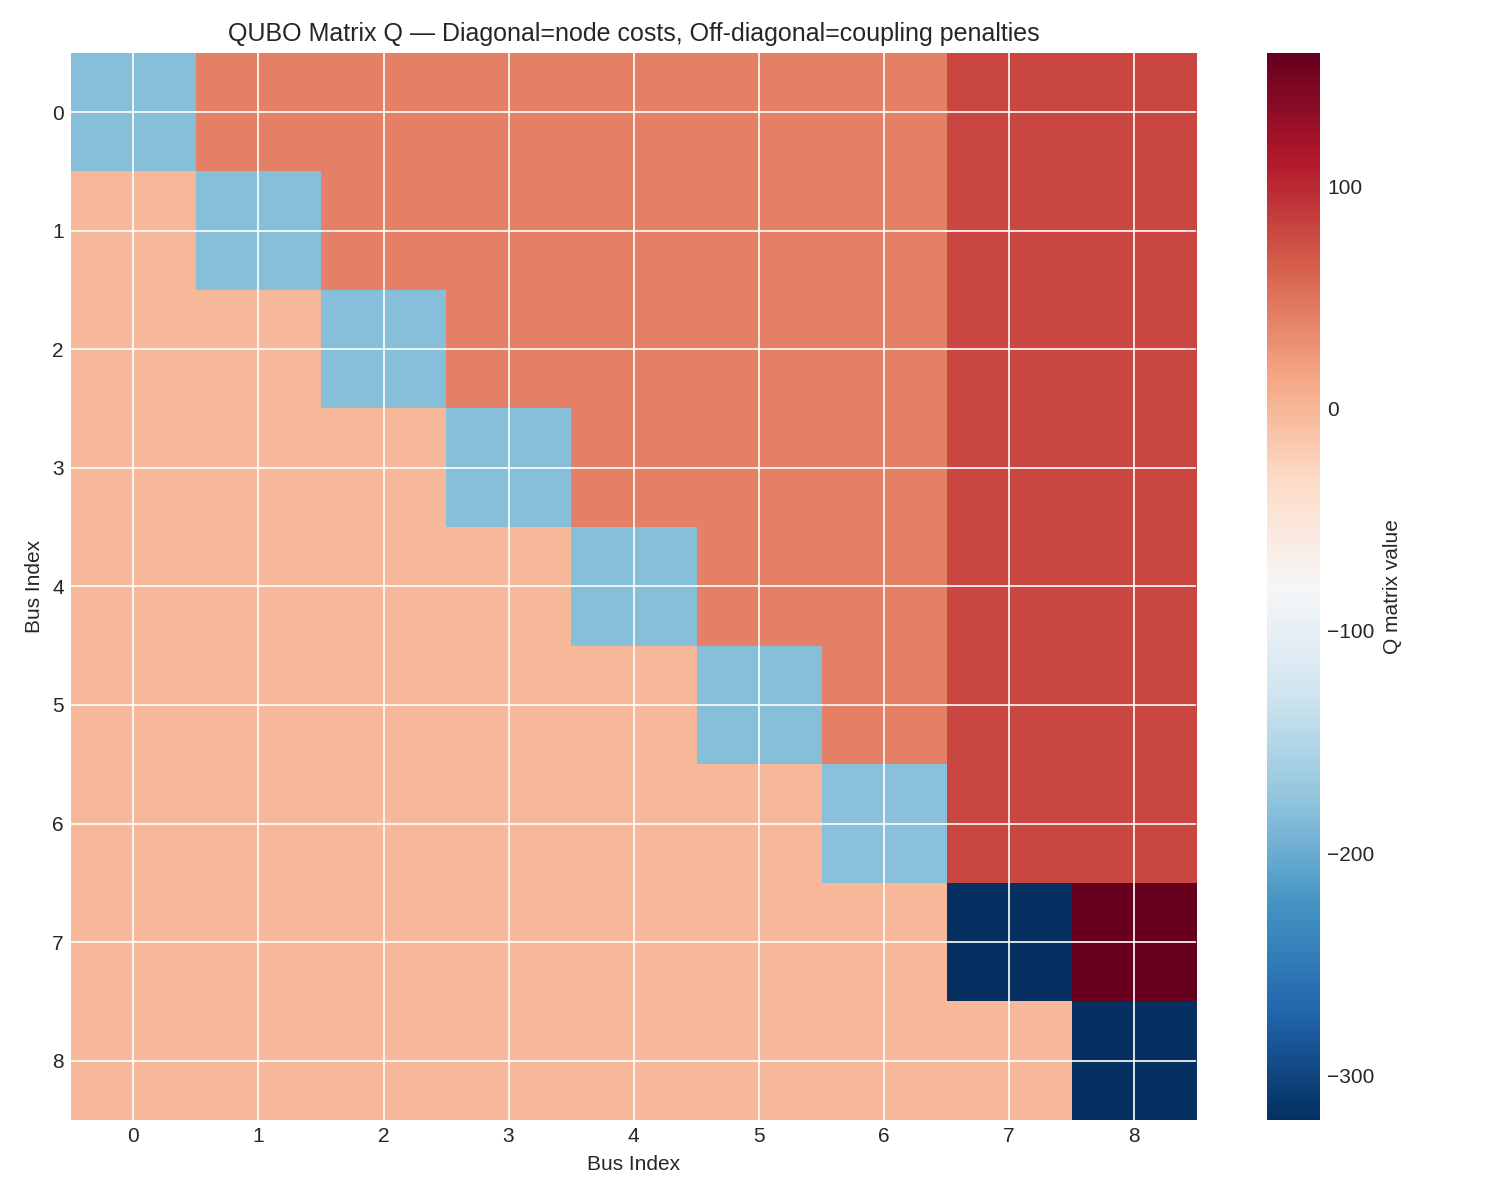
\includegraphics[width=0.95\columnwidth]{../images/04_qubo_matrix.png}
    \caption{Q-Matrix displaying dense off-diagonal penalty allocations required by local budget capacities.}
\end{figure}

\section{Optimization Results}
Executing local Qiskit hybrid solvers evaluated algorithmic convergence accuracy at low gate depths ($p=1$). Validating these outputs against PuLP mapped CBC implementations yields physical confidence limits validating the exact ratios.

\begin{figure}[H]
    \centering
    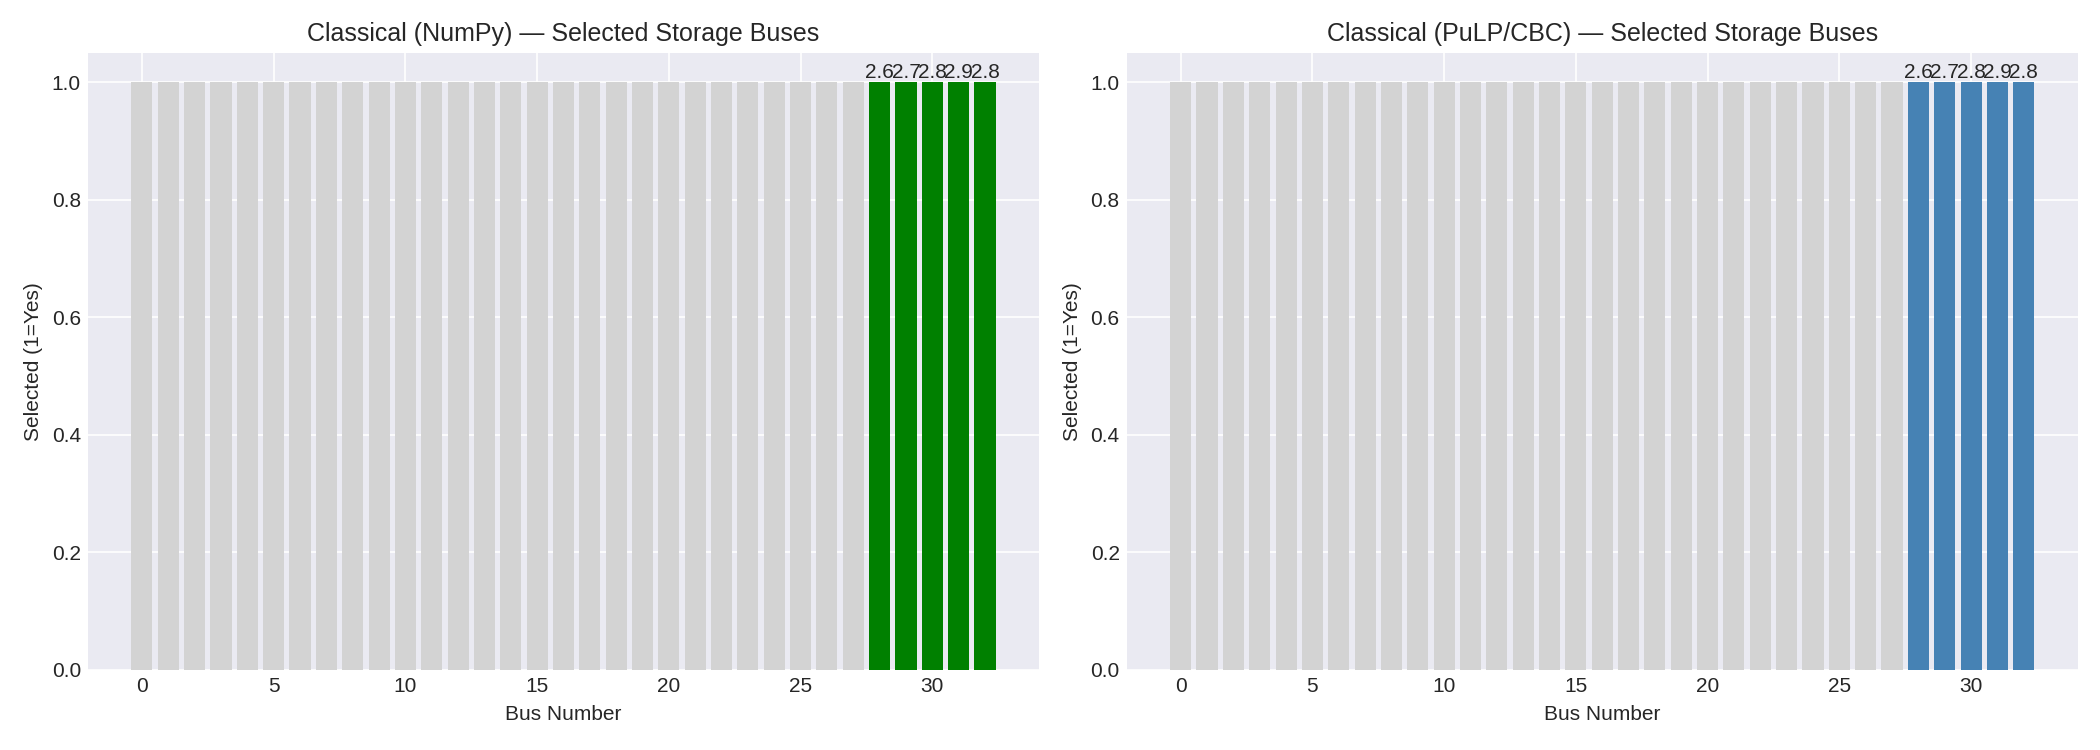
\includegraphics[width=0.95\columnwidth]{../images/05_classical_solutions.png}
    \caption{NumPy vs PuLP exact solver BESS placements.}
\end{figure}

\begin{figure}[H]
    \centering
    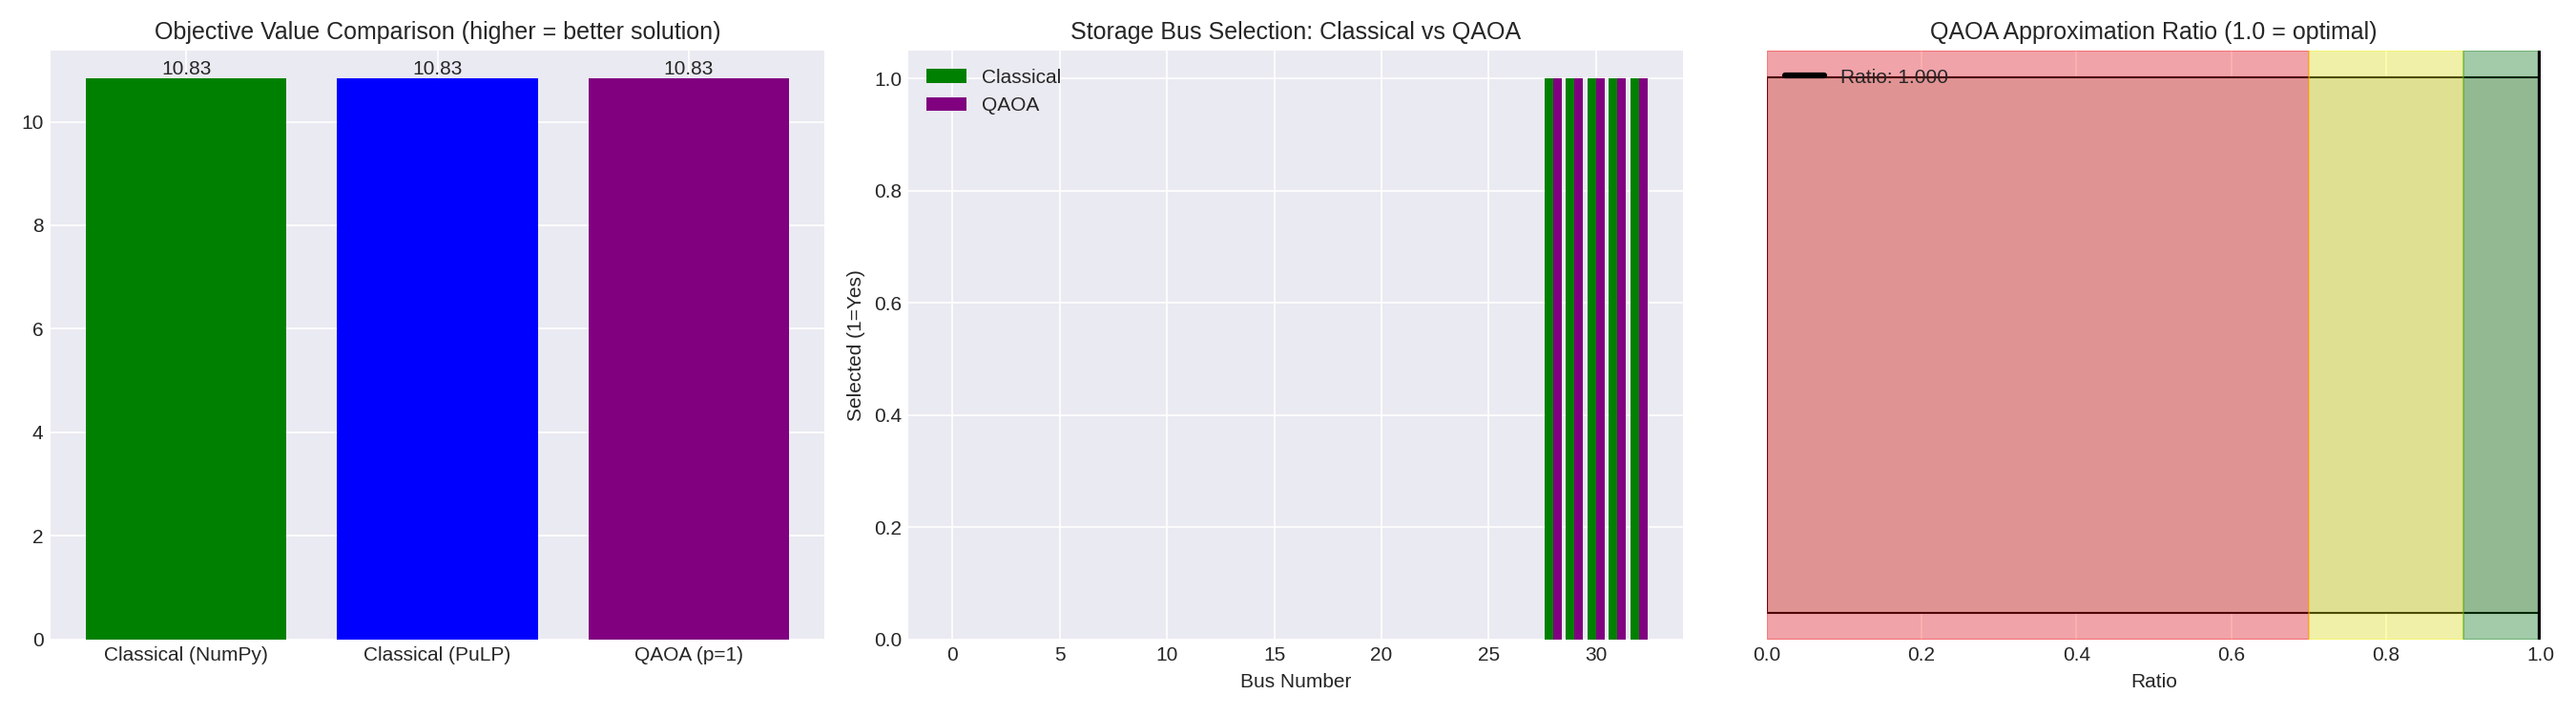
\includegraphics[width=0.95\columnwidth]{../images/06_qaoa_results.png}
    \caption{QAOA parameter convergence profiling showing a matched Approximation Ratio.}
\end{figure}


\section{Grid Physics Validation}
Post-allocation, validation environments scaled inputs to an independent \texttt{pandapower} grid instance injecting 0.3 MW BESS components per optimal integer parameter. 

The reverse power-flow bounds strictly validate real-world operational benefits without risking distribution line failure. Optimal sites mathematically lifted average distribution voltage bounds from 0.913 to 0.935 pu.

\begin{figure}[H]
    \centering
    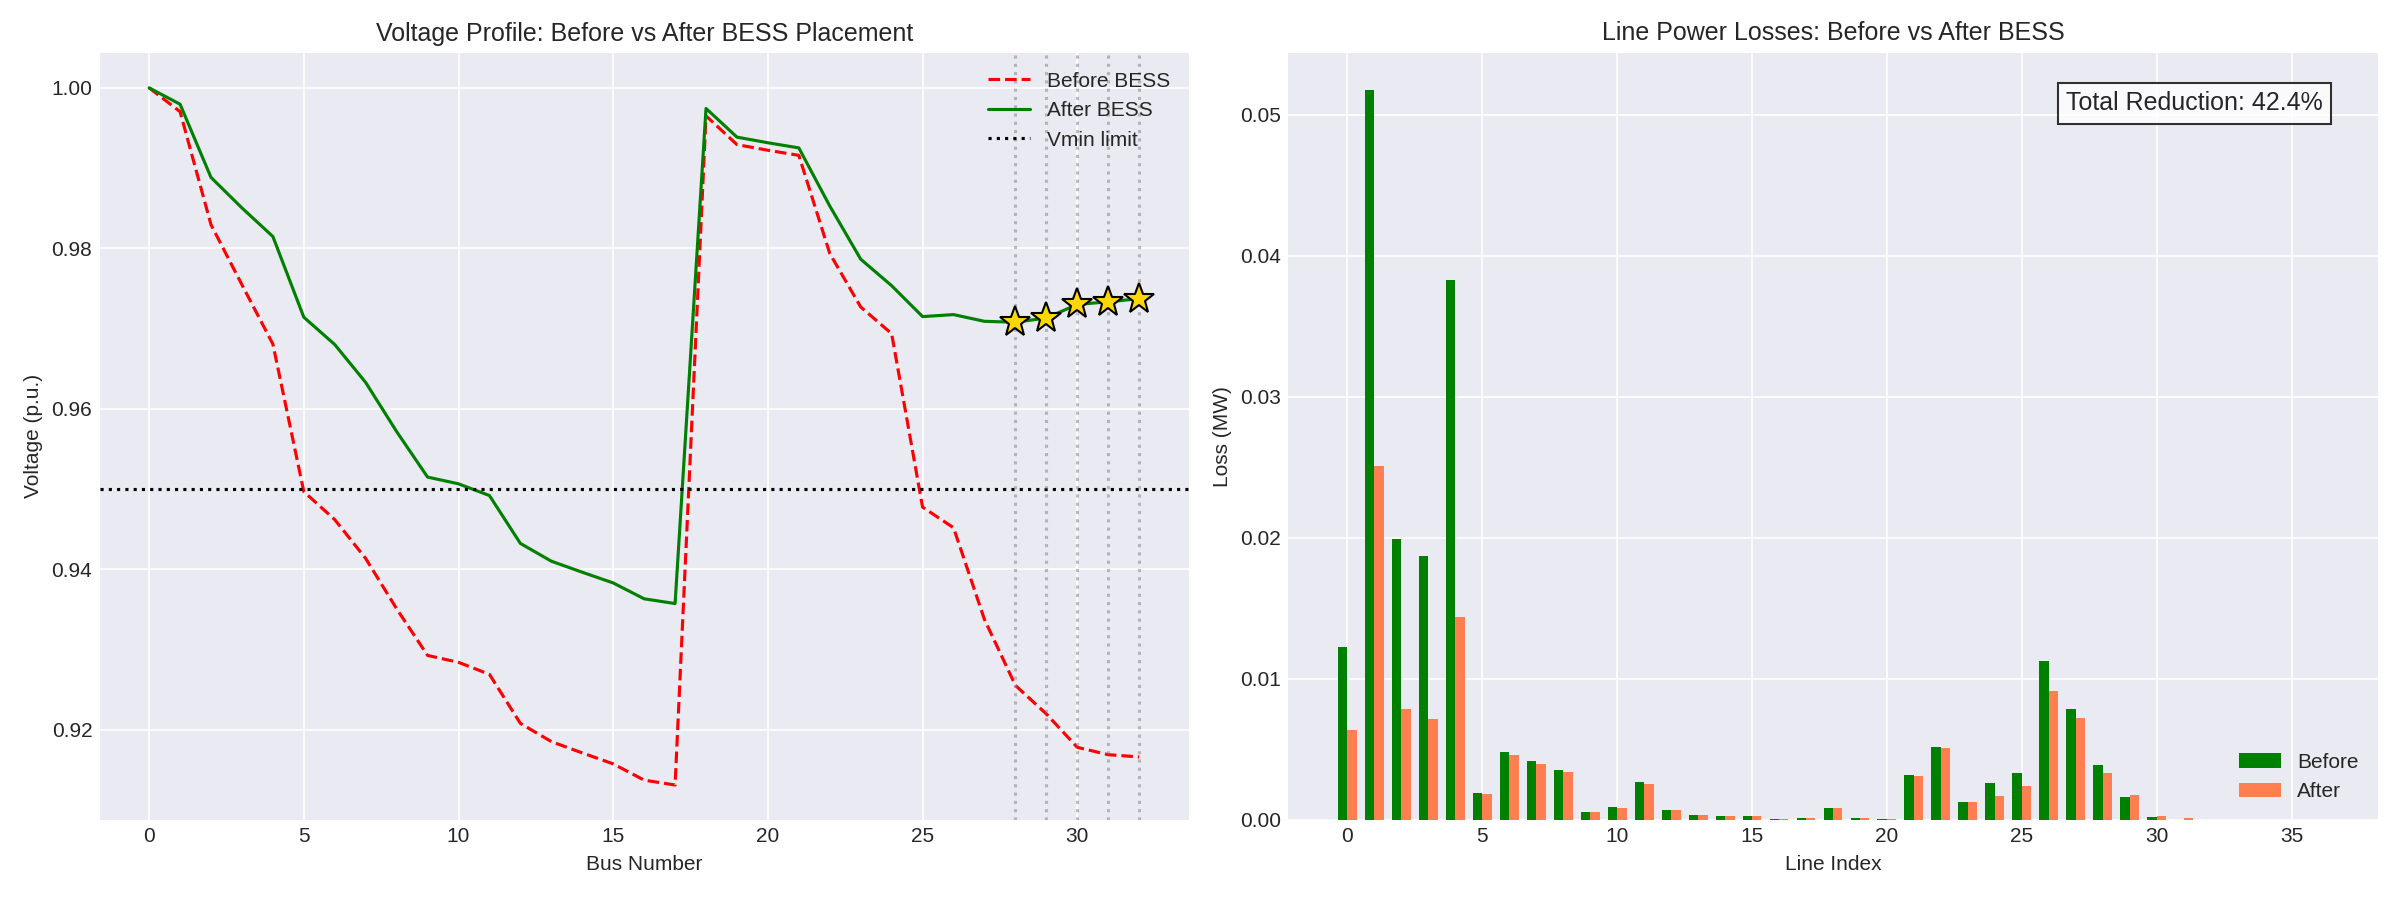
\includegraphics[width=0.95\columnwidth]{../images/07_validation_results.png}
    \caption{Grid voltage and loss profiles before and after BESS allocation.}
\end{figure}


\section{Scalability and Quantum Advantage Projection}
Combinatorial optimization frameworks demonstrate bounded execution thresholds matching polynomial $O(p \times n)$ scaling profiles structurally capable of surpassing exponential state bounds limits.

\begin{figure}[H]
    \centering
    \includegraphics[width=0.95\columnwidth]{../images/08_scaling_analysis.png}
    \caption{Extrapolation charting of algorithm execution limits vs classical scaling limits.}
\end{figure}

\begin{figure}[H]
    \centering
    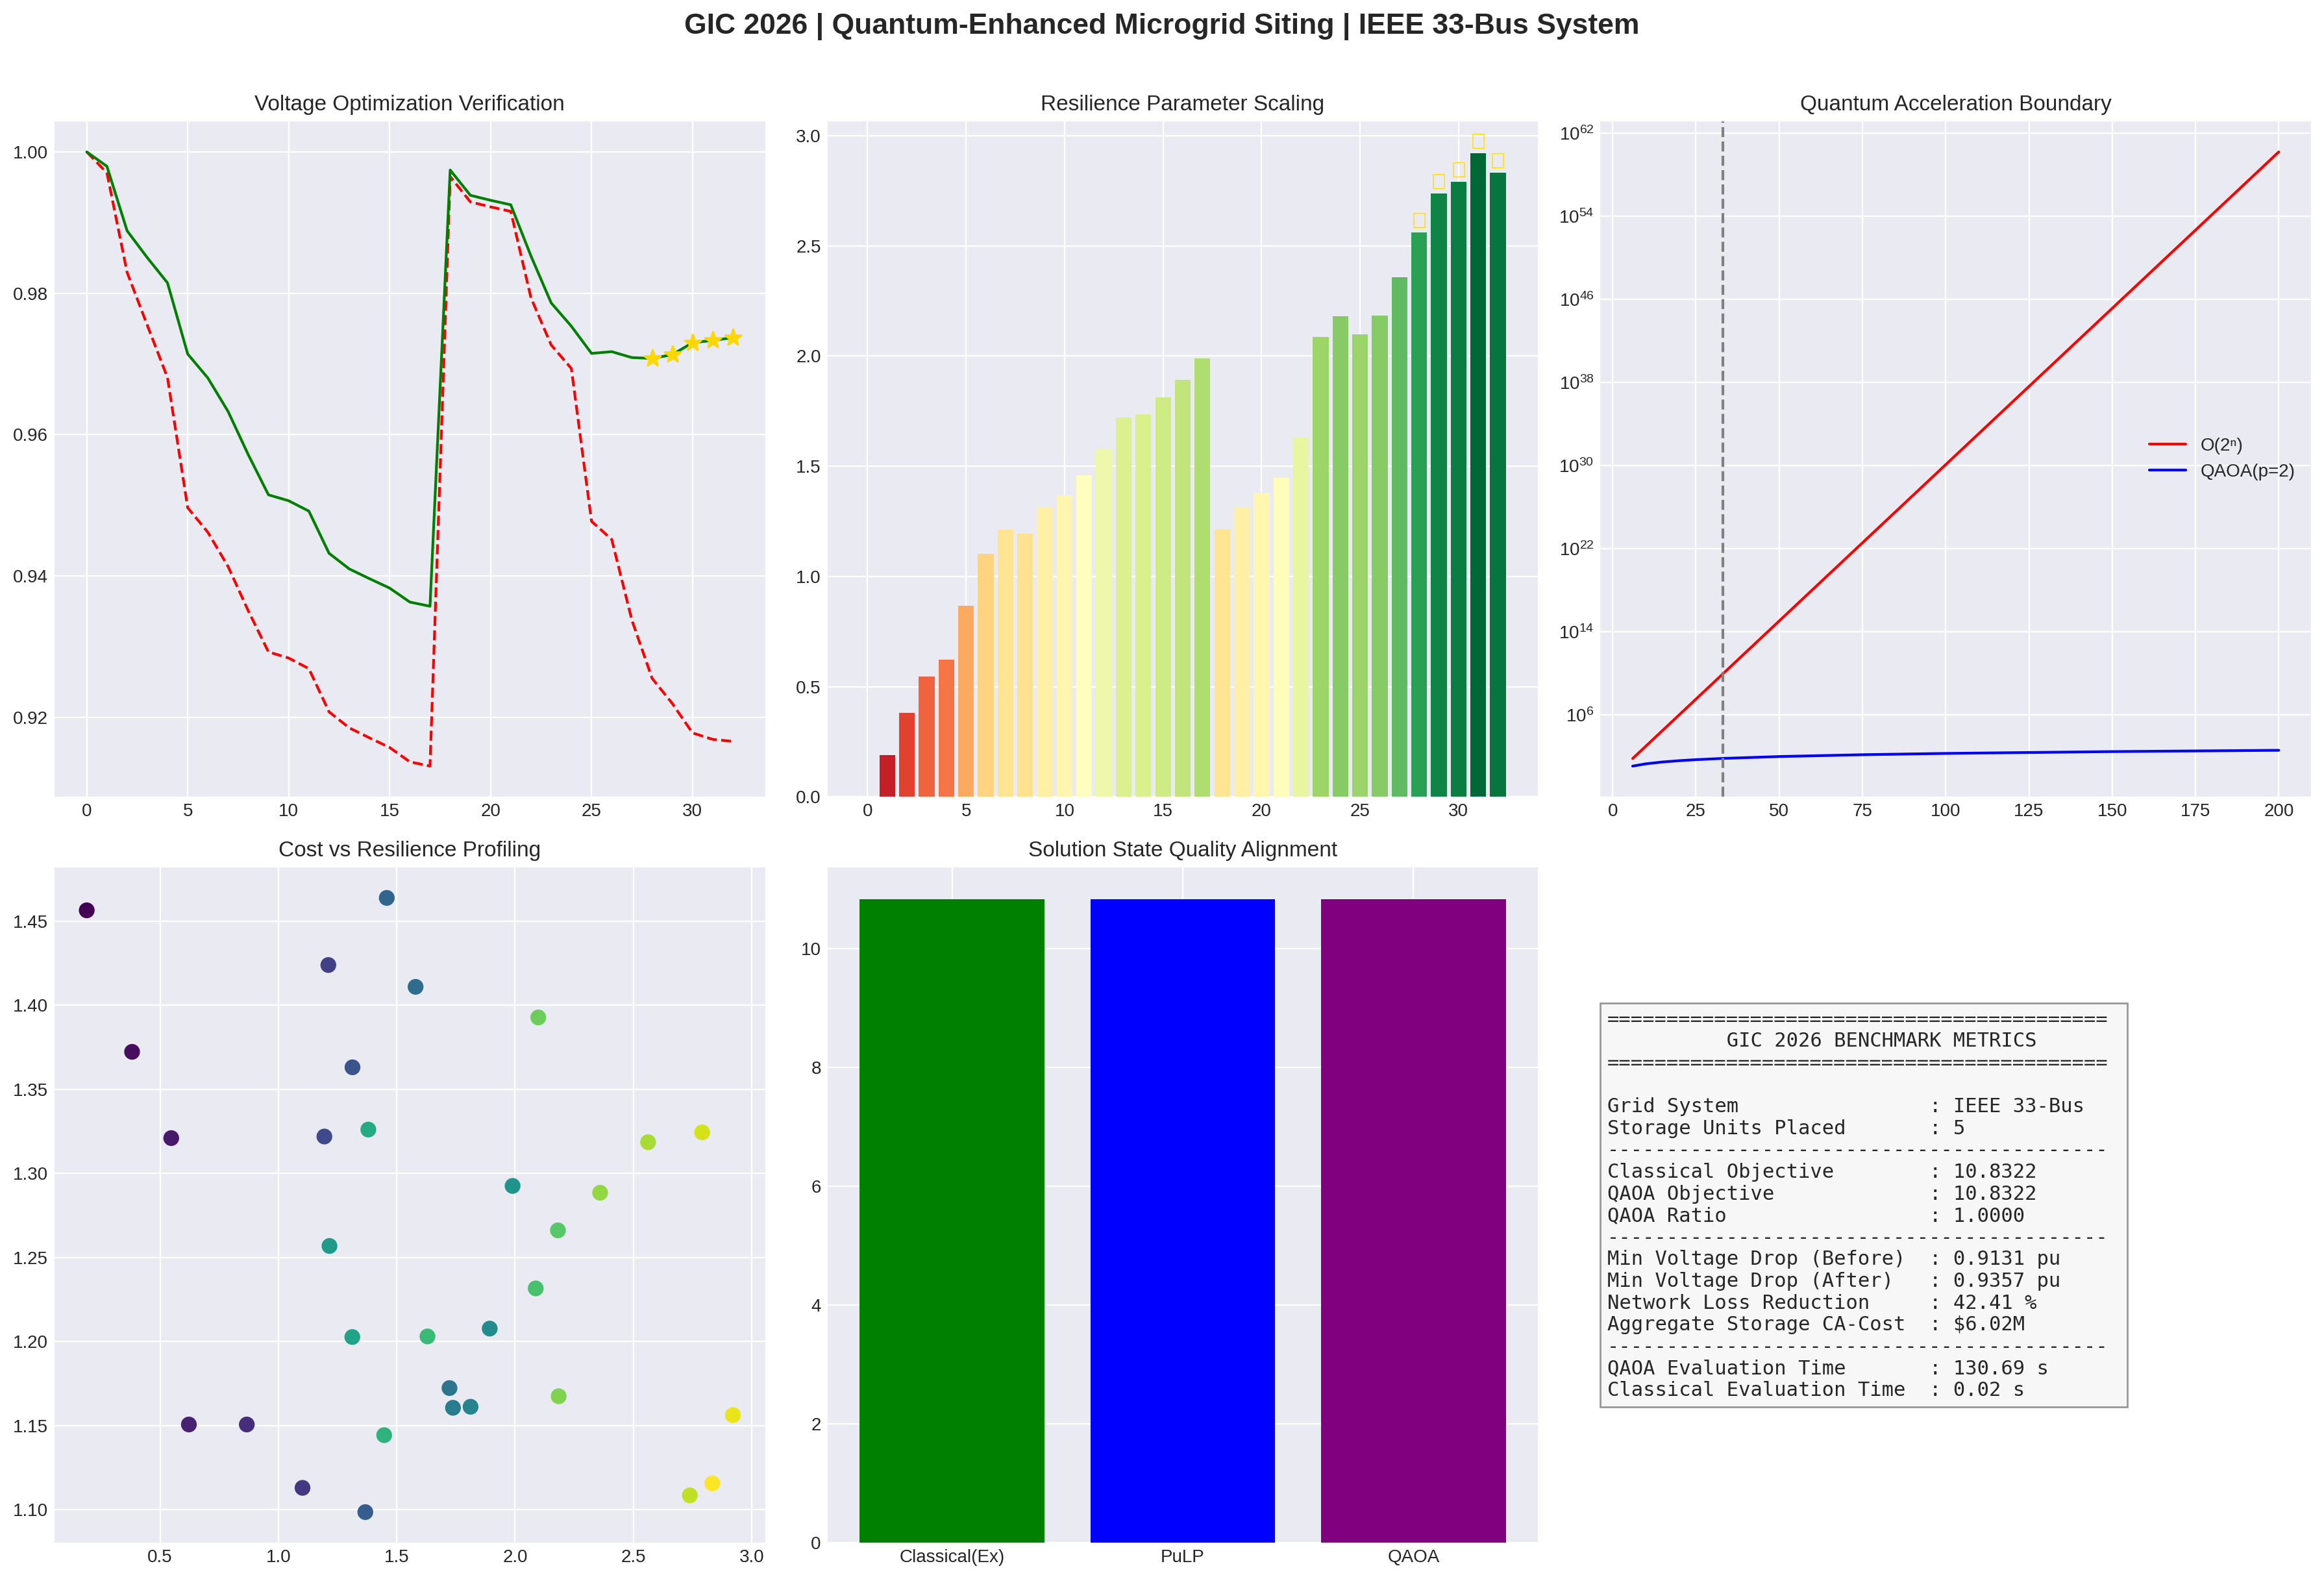
\includegraphics[width=0.95\columnwidth]{../images/09_final_dashboard.png}
    \caption{Macro view consolidating grid validation, performance tracking, and convergence success parameters.}
\end{figure}


\section{Future Improvements to the Model}
While this hybrid architecture securely proved mathematical tractability mapping a 33-bus system constraint into the Quantum Approximate Optimization Algorithm (QAOA), several advanced modeling enhancements can extend limits for large-scale operation profiles:

\begin{enumerate}
    \item \textbf{Transition to Large-Scale Topologies (IEEE 118-Bus):} Scaling nodes proportionally drives polynomial optimization density limits. Executing the QUBO formulations against a larger graph requires advanced modular mapping patterns to sidestep full-connectivity matrix densification bottlenecks \cite{pnnl2024emerging}.
    
    \item \textbf{Accelerated Benders Decomposition (ABD) Integration:} To break NP-hard dependencies for generalized utility applications, coupling the QUBO framework into hybrid Benders decomposition models resolves execution limits splitting optimal flow models classically while rendering allocation integer choices on Quantum environments structurally \cite{ellinas2024hybrid}.
    
    \item \textbf{Hardware Error Mitigation and Physical Deployment:} Future integration must transition testing metrics outside simulated statevector envelopes (\texttt{StatevectorSampler}) targeting real cloud IBM Quantum nodes directly. Implemented noise-filtering methods using Readout-Error Mitigation strategies will adapt physical constraint logic cleanly against stochastic gate faults.
    
    \item \textbf{Financial Multi-Scenario Uncertainty Vectors:} Real market loads exhibit variance gradients over extended solar-cycles. Implementing probabilistic Monte Carlo analysis dynamically scales $r_i$ parameters yielding predictive optimization vectors targeting real resilience profiles under climate disruptions structurally resolving true ISO constraints \cite{morstyn2024quantum}.
\end{enumerate}

\nocite{*}
\bibliographystyle{ieeetr}
\bibliography{references}

\end{document}
